

\inlineanswer{All four runs used the same training batches, batch size (16),
gradient clipping threshold (1), and random seed (42). Each row retains the
previous row's changes. The loss shown is for the batch used in update 100.}

\begin{center}
\begin{tabular}{lrrr}
\toprule
Run & Learning rate & AdamW $\beta_2$ & Width \quad Loss \\
\midrule
Baseline & $10^{-5}$ & 0.999 & $33 \qquad 10.7784$ \\
1. Higher learning rate & $3\times10^{-3}$ & 0.999 & $33 \qquad 4.9214$ \\
2. Faster second moment & $3\times10^{-3}$ & 0.95 & $33 \qquad 4.9105$ \\
3. Wider model & $3\times10^{-3}$ & 0.95 & $96 \qquad 4.8148$ \\
\bottomrule
\end{tabular}
\end{center}

\inlineanswer{A higher learning rate lets the model take larger updates early
in training. Lowering $\beta_2$ lets AdamW's squared-gradient estimate react
more quickly over a short run. Increasing the model width gives each token
more features while keeping the number of heads and layers fixed. The lowest
step-100 loss was \textbf{4.8148}. The optimizer change produced only a small
improvement in this run; these curves do not establish a gain across seeds.}

\noindent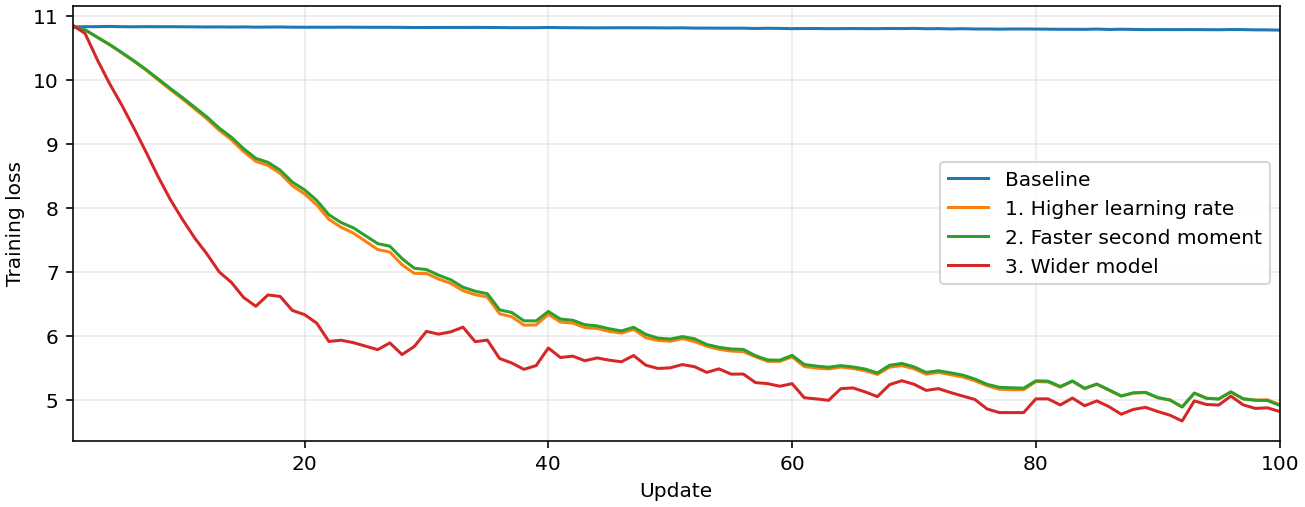
\includegraphics[width=\linewidth]{a3-bonus.png}\par
